%  Beamer slide example.

\documentclass[9pt]{beamer}
\usepackage[utf8]{inputenc}
\usetheme{inria}
\usepackage{helvet}
\usepackage{graphicx}
\usepackage{nameref}

\author{Maurice Bremond \and Gaëtan Harter}

\title[Intégration continue]{L'Intégration Continue}
% \subtitle{Dans un contexte de développement Inria}
\subtitle{Présentation IJD}

% Automatically insert a "new section" page at each section.
\AtBeginSection[]{
  \begin{frame}[plain]
    \partpage
  \end{frame}
}
% \inriaswitchcolors COLOR
%
% Where COLOR is one of red, blue, orange, darkblue, violet,
% pastelgreen, grey, or green.
\newcommand{\inriaswitchcolors}[1]{%
  \pgfaliasimage{figfootline}{figfootline-#1}% !!!
  \pgfaliasimage{figbackground}{figbackground-#1}% !!!
  \pgfaliasimage{figbackground}{figbackground-#1}% !!!
}

% frame with toc for current subsection
\newcommand{\tocsubsection}{
  \begin{frame}
    \tableofcontents[
      currentsubsection,
      sectionstyle=show/shaded,
      subsectionstyle=show/shaded,
      subsubsectionstyle=show/show/shaded
    ]
  \end{frame}
}
% starting the document
% *********************
\begin{document}
% titlepage
% ---------
\begin{frame}[plain]
  \titlepage
\end{frame}
% table of contents
% -----------------
\begin{frame}{\textcolor{inriaGrey}{Table des matières}}
  \tableofcontents
\end{frame}



% Introduction
% ************

\inriaswitchcolors{red}
\section{Quid de l'intégration continue}

\subsection{Qu'est-ce que c'est}
\begin{frame}{\subsecname}

  Contenu

\end{frame}



% L'intégration continue à Inria
% ******************************
\inriaswitchcolors{blue}
\section{L'intégration continue à Inria}




% Retour d'expérience
% *******************
\inriaswitchcolors{green}
\section{Un retour d'expérience}
\frame{\tableofcontents[currentsection]}

\subsection{Contexte de développement}
\tocsubsection

\subsubsection{Plateforme de réseau de capteurs: FIT IOT-LAB}
\begin{frame}{\subsubsecname} %{\subsecname}
  \setbeamercovered{transparent}
  \begin{itemize}
    \item <2->{Plateforme de réservation et expérimentation pour matériel réseau sans fil}
    \item <2->{Utilisé par des chercheurs depuis leur bureau}
    \item <2->{Déploiement à large échelle, 3000 nœuds capteurs}
    \item <2->{Projet d'une durée de 10ans}
  \end{itemize}
  \onslide <3-> ~\\~\\ Réservation, configuration et mise à disposition de nœuds capteurs.
\end{frame}


\begin{frame}{\subsubsecname} %{\subsecname}

  IMAGE DE LA PLATEFORME COMPLETE

\end{frame}

\subsubsection{Contexte de l'application}
\begin{frame}{\subsubsecname} %{\subsecname}
  \begin{itemize}
    \item Application mise en production
    \item Exécution sur une carte ARM avec Linux embarqué (perf...)
    \item Commande par interface REST (web)
    \item Interaction par port série avec un OS temps réel sur un micro-contrôleur
    \item multithread, multiprocess
    \item Il faut préserver les interfaces à tout moment
  \end{itemize}
\end{frame}


\subsubsection{Pourquoi avoir mis place de l'intégration continue}
\begin{frame}{\subsubsecname} %{\subsecname}
  \begin{itemize}
    \item Une pratique qui m'intéresse
    \item Logiciel final doit être fiable
    \item Source d'erreurs aléatoires
    \item Déployé à large échelle
  \end{itemize}
\end{frame}



\subsection{Outils mis en place}
\tocsubsection

\subsubsection{Présentation des outils}
\begin{frame}{Outils mis en place}

  Gestionnaire de versions: \texttt{git} \\ ~ \\

  \begin{tabular}{ l | l l | p{3.5cm} }
    Language         & \texttt{Python}     & \texttt{C}    & Utilisation dans Jenkins \\ \hline
    Script de build  & \texttt{setuptools} & \texttt{Make} & Bash~shell, \texttt{EnvInject} \texttt{virtualenv}\\
    Compilation      & ~                   & \texttt{gcc}  & ~ \\
    Tests            & \texttt{unittest}, \texttt{mock}, \texttt{nose}
                     & \texttt{gtest} \texttt{(C++)}
                     & Junit, Chuck Norris\\
    Couverture       & \texttt{nose-xcover}
                     & \texttt{gcov}, \texttt{gcovr}
                     & Cobertura \\
   Qualité de code  & \texttt{pylint}, \texttt{pep8} & ~  & Violations \\
    ~ & ~  & ~ & \\
    Lignes de code   &  $3000$        &  $1500$  &  $0$  \\
    Lignes de tests  &  $1600 + 400$  &  $1300$  &  $0$  \\
% 1600 tests U + 400 tests intégration
    Lignes de build  &  $300$         &  $170$   &  $50$ \\

% (SQLite 3.8 == 1084 * plus de tests que de code 84k source (hors blank et commentaires))
  \end{tabular}
\end{frame}


\subsubsection{Jenkins}
\begin{frame}{Présentation outils}{Jenkins}
  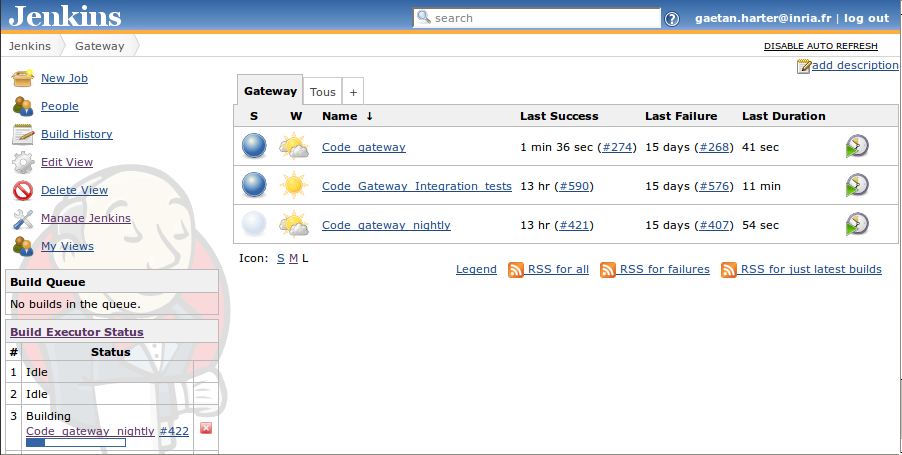
\includegraphics[width=\linewidth]{images/jenkins}
\end{frame}

\begin{frame}{Configuration d'un build}{Jenkins}
  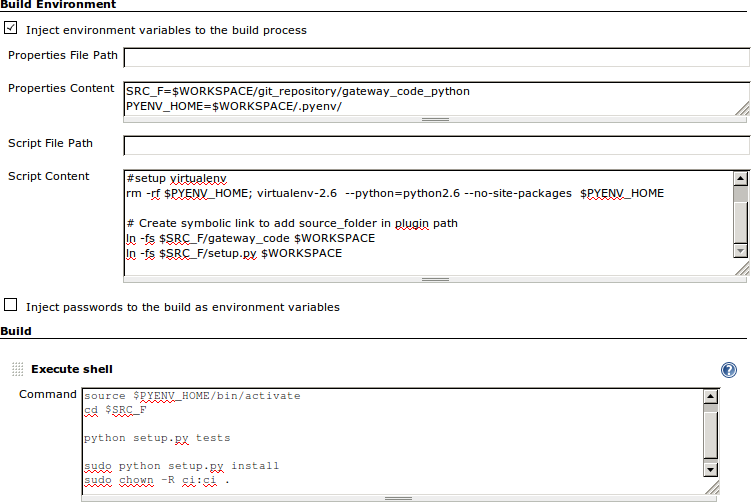
\includegraphics[width=\linewidth]{images/build_configuration}
\end{frame}


\begin{frame}{Cobertura}{Jenkins}
        % Pour moi, l'outil le plus important (après Chuck Norris forcément)
  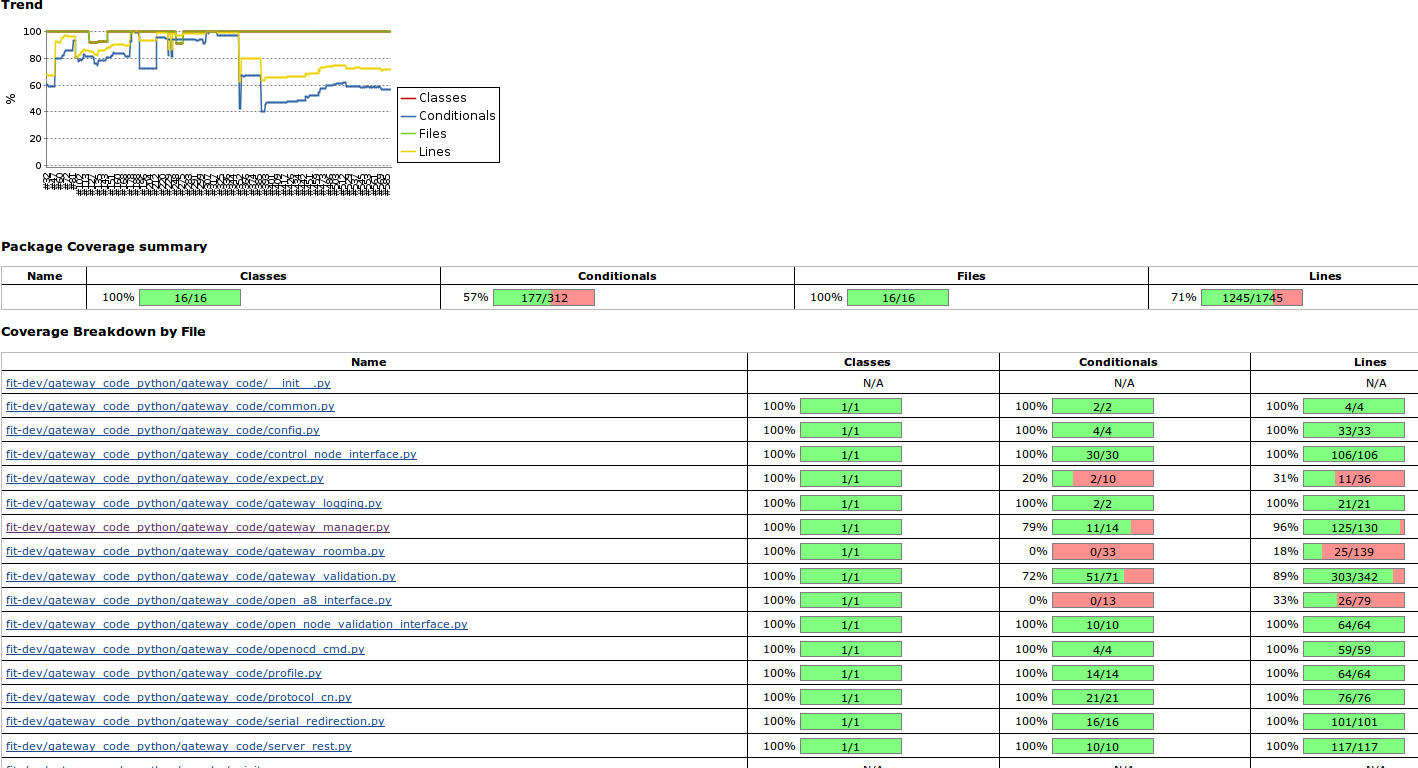
\includegraphics[width=\linewidth]{images/cobertura}\\
\end{frame}
\begin{frame}{Junit - Violations}{Jenkins}
  \begin{center}
        % Juste pour montrer
    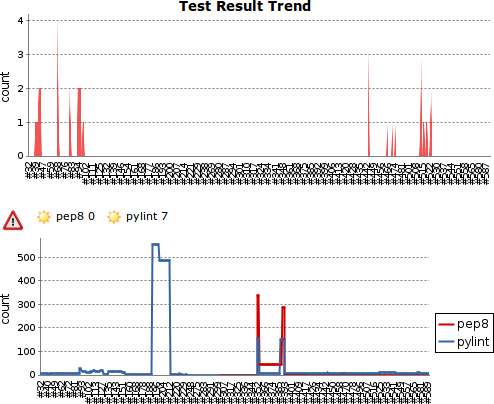
\includegraphics[height=0.8\textheight]{images/junit_violations}\\
  \end{center}
\end{frame}
\begin{frame}{Chuck Norris}{Jenkins}
  % Le plus important des plugins
  \begin{center}
    \begin{tabular}{ l |l }
      Build KO & Build OK \\ \hline
        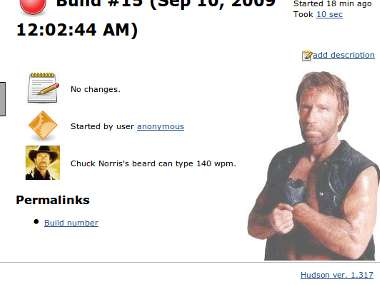
\includegraphics[height=4cm]{images/chuck_full} &
      
\includegraphics[height=4cm]{images/chuck_happy}
        %
\includegraphics[height=4cm]{images/chuck_angry}
      \\
    \end{tabular}
  \end{center}
  Chuck Norris Facts:
  \begin{itemize}
    \item Chuck Norris can unit test an entire application with a single assert.
    \item Chuck Norris can divide by zero.
    \item ...
  \end{itemize}
\end{frame}




\subsection{Bilan}
\tocsubsection


\subsubsection{Développement logiciel}
\begin{frame}{\subsubsecname}{\subsecname}
  \setbeamercovered{transparent}

  \begin{itemize}
    \item <2-> Mise en place d'un script de \texttt{build}
      \begin{itemize}
        \item Mise en place d'une procédure de test (pouvoir écrire et lancer un test)
        \item Procédure simple et conditionnée dans un script
      % \item Adhérence aux conventions d'architecture du language
      \end{itemize}
    \item <3->Tests nombreux et lancés en continue
      \begin{itemize}
        \item Apparition et gestion des cas d'erreurs (cas 'rares')
        \item Détection de problèmes tot (performance, permissions)
        \item Simplification de l'implémentation pour la testabilité
        \item Ajout au fur et à mesure des fonctionnalités (non régression)
      % \item Suivi des bugs
      \end{itemize}
    \item <4-> Couverture de code
      \begin{itemize}
        \item Même si $<100\%$, savoir ce qui est 'validé' et ce qui ne l'est pas
      \end{itemize}
    \item <5-> Qualité de code (Python)
      \begin{itemize}
        \item Remplace la phase de compilation (vérification syntaxique)
        \item Détection statique d'erreurs
        \item Standardisation de la mise en forme, lisibilité (PEP8)
      \end{itemize}
  \end{itemize}
  \onslide <6-> Maîtrise et confiance dans le logiciel développé
\end{frame}

\subsubsection{Personnel}
\begin{frame}{\subsubsecname}{\subsecname}
  \begin{itemize}
    \item Découverte de beaucoup d'outils
    \item Confort dans le développement (non régression)
    \item Retours positifs après premières utilisations
  \end{itemize}
\end{frame}

\subsubsection{Voies d'amélioration}
\begin{frame}{\subsubsecname}{\subsecname}
  \begin{itemize}
    \item Passer les configurations Jenkins dans des scripts versionnés
    \item Grouper Python et C dans le build python
    \item Inclusion d'autres développeurs
    \item 100\% de couverture de code
  \end{itemize}
\end{frame}

\end{document}
